\documentclass[a4paper,11pt]{article}
\usepackage[utf8]{inputenc}
\usepackage[T1]{fontenc}
\usepackage[french]{babel}
\usepackage{makeidx}
\usepackage{textcomp}
\usepackage{graphicx}
\usepackage{mathtools,amssymb,amsthm}
\usepackage{lmodern}
\usepackage{multirow}
\usepackage{array}
\usepackage{longtable}

\title{TER 2019 - Spécifications}
\author{Maxime Gonthier - Benjamin Guillot - Laureline Martin}
\begin{document}
	\pagenumbering{gobble}\clearpage
	\maketitle

\newpage
\tableofcontents

\newpage
\section{Introduction}
Dans la société actuelle, les transports en communs prennent une part de plus en plus importante dans nos déplacements. Bien que pratique et plus écologique, ils sont toujours relativement pleins et donc peu agréable.\\
 L'un des objectifs d'un bureau des temps est de réduire la congestion à l'intérieur de ces transports, c'est à dire de réduire le nombre de personnes présentent en même temps dans un transport. 
Notre objectif est donc de faire ce travail en partant d'un cas concret, celui de la ligne de bus R reliant la gare de Versailles-Chantier à l'Université Versailles-Saint Quentin. Pour ce faire, nous allons influer sur les emplois du temps de l'Université en modifiant les heures de début de cours sur une journée afin de voir si la congestion est susceptible de baisser au niveau de la ligne de bus après ces modifications.\\
A la fin du projet, le but est de fournir une planification de l'emploi du temps de l'Université sur une journée, c'est-à-dire les débuts de chaque cours.

\section{Modélisation des données en entrée}
	Nous répartissons les données concernant la l'Université en 5 modules.\\
	Un module est constitué d'une classe et de fonctions nécessaire à la modélisation d'un acteur essentiel du projet. Par la suite, les modules seront reliées entre eux et s'appelleront mutuellement.
	\begin{itemize}
		\item Module cours
		\item Module salle d'enseignement
		\item Module étudiant
		\item Module professeur
		\item Module bus
	\end{itemize}

	\subsection{Module Cours}
		Le module cours est une classe représentant un cours sur un temps donné.\\
		Lors des affectations, on modifiera l'horaire de début pour chaque instance à déplacer.\\
		\subsubsection{Classe Cours}
		\begin{enumerate}
			\item num\_cours :  un entier (identifiant unique)
			\item duree : un entier (représente la durée du cours en minutes)
			\item liste\_etu : un tableau d'entiers qui contient les numéros des étudiants participant à ce cours. On calcule le nombre d'étudiants participant au cours à partir de cette liste.
			\item type\_salle : un entier, 0 pour une salle de TP et 1 pour un autre salle (on pourra ajouter d'autres types de salle si nécessaire).
			\item num\_salle : un entier (identifiant unique représentant la salle)
			\item num\_ens : un entier désignant le professeur donnant ce cours(identifiant unique représentant le professeur)
			\item debut : un entier. On divise le temps d'ouverture de l'Université en créneaux de 15 minutes, chaque entier représente le début d'un bloc de 15 minutes. 
			\item liste\_ens : une liste contenant les identifiants des professeurs pouvant enseigner ce cours.
		\end{enumerate}

	\subsection{Module Salle d'enseignement}
		Le module salle représente la localisation du cours sur un temps donné.
		\subsubsection{Classe Salle}
		\begin{enumerate}
			\item num\_salle : un entier (identifiant unique)
			\item localisation : un entier, 0 pour proche de l'arrêt de bus desservant l'Université, 1 pour modérément éloigné, 2 pour éloigné. 
			\item type\_salle : un entier, 0 pour une salle de TP et 1 pour une autre salle (on pourra ajouter d'autres type de salle si necessaire).
			\item capacite : un entier désigant le nombre maximal d'étudiants que peut contenir la salle	
		\end{enumerate}
		\subsubsection{Matrice d'adjacence entre les salles}
			Cette matrice permet d'indiquer la distance entre deux salles. Matrice symétrique.\\ 0 Si la distance à parcourir à pieds est inférieure à 15 min, 1 si la distance est comprise entre 15 et 30 min, 2 sinon.
		\subsubsection{Matrice d'adjacence entre salles et arrêt de bus}
			Matrice colonne représentant la distance entre l'arrêt de bus desservant l'Université et les salles. On regarde le temps à parcourir à pieds entre l'arrêt de bus et la salle et on remplit de la même manière que pour la matrice précédente.
	\subsection{Module Etudiant}
		Le module étudiant représente un étudiant.
		\subsubsection{Classe Étudiants}
		\begin{enumerate}
			\item num\_etu : un entier (identifiant unique)
			\item distance : un entier, représente la distance entre le domicile de l'étuidant et l'Université, 0 si l'étudiant habite à moins de 15 min de la l'Université, 1 s'il habite entre 15 et 45 min, 2 sinon.
			\item contrainte : un entier, représente la contrainte faible à laquelle un étudiant peut être associé. 0 s'il n'est associé à aucune contrainte, 1 s'il associé à la contrainte travail, 2 s'il est associé à la contrainte enfant, 3 s'il est associé aux deux contraintes précédentes. 
			\item heure\_debut : un entier, représente l'heure du premier cours de la journée de l'étudiant.
			\end{enumerate}
	\subsection{Module Enseignant}
		Le module Enseignant représente un enseignant.
		\subsubsection{Classe Enseignant}
		\begin{enumerate}
			\item num\_ens : un entier (identifiant unique)
			\item plage : un tableau dont chaque case représente un bloc horaire (15 min par exemple). Si $x_i$ vaut 0 alors c'est l'horaire du début de la disponibilité, si $x_i$ vaut 1 c'est la fin de la disponibilité de l'enseignant.
			\end{enumerate}

	\subsection{Module Bus}
		Pour les transports, on supposera que chaque élève arrivera par le bus précédant le début du premier cours de sa journée. De cette manière, à chaque itération de l'affectation des cours, on pourra recalculer la congestion de chaque bus (qui sera utilisé comme fonction objectif du projet une fois les transport implémentés).\\
		La congestion sera représentée par le maximum du dépassement de la limite de confort du bus lors du trajet. On utilisera la fonction "calcul congestion" décrite ci-dessous pour calculer cette valeur pour chaque bus. On pourra représenter un bus de la façon suivante :
		\begin{itemize}
			\item liste\_arrêt : une liste de tous les arrêts par lequel passe le bus. Pour chaque arrêt, on aura le nombre de personne entrantes et sortantes du bus.
			\item seuil\_confort : un entier, représente le nombre de personnes que peu contenir le bus avant que la fréquentation ne devienne désagréable pour les usagers.
			\item capacité\_max : un entier, représente le nombre maximum de personnes pouvant être dans le bus en même temps.
		\end{itemize}

	\subsection{Liens entre les modules}
		\centerline{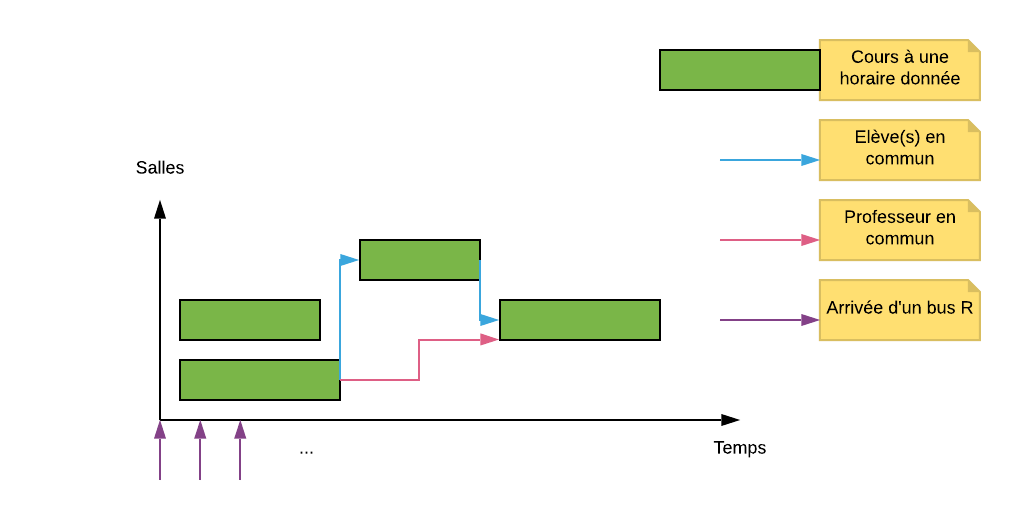
\includegraphics[scale=0.5]{modelter.png}}
		Modélisation graphique des données en entrées.\\

\section{Modélisation des Contraintes}
	Pour optimiser, nous faisons face à plusieurs contraintes, toutes ne sont pas 
	de même "importances". Nous allons donc devoir définir un ordre de priorité sur 
	les contraintes, ainsi lors de l'optimisation par notre algorithme, nous 
	pourrons ajuster et obtenir de meilleurs résultats même si certaines contraintes
	"faibles" sont violées.\\
	\subsection{Contraintes dures}
			\subsubsection{Entre deux cours}
				\begin{enumerate}
					\item Deux cours utilisent la même salle ne doivent pas avoir des horaires qui se chevauchent
					\item Deux cours qui ont des horaires qui se chevauchent ne doivent pas avoir d'élèves en commun.
					\item Le temps laissé entre deux cours ne peut pas être inférieur au temps nécessaire pour relier les deux salles.
				\end{enumerate}
			\subsubsection{Entre un cours et un professeur}
				\begin{enumerate}
					\item Le professeur doit pouvoir enseigner ce cours (d'où la création de la liste de professeurs pouvant enseigner un cours dans le module cours).
					\item La plage de disponibilité du professeur correspond à l'horaire du cours.
				\end{enumerate}
			\subsubsection{Entre un cours et une salle}
				\begin{enumerate}
					\item 	La salle doit avoir une capacité supérieure ou égale au nombre d'élèves suivant le cours et doit correspondre au type de salle dont le cours a besoin.
				\end{enumerate}
			\subsection{Pour un Bus}
				\begin{enumerate}
					\item Le nombre d'étudiants $E$ ne doit pas dépasser la capacité $capacité_{max}$ du bus.
				\end{enumerate}
	On ne précise pas la contrainte entre cours et étudiant car un étudiant est défini par ses cours.
	\subsection{Contraintes faibles}
		\begin{enumerate}
			\item Avoir une personne à charge ce qui impose un horaire le matin et/ou le soir. Exemple : Soit X, l'heure de début d'un cours, si un enfant doit être déposé à l'école à 9h on a : X > 9 + (indice de distance de cet étudiant)*30 min. Soit Y, l'heure de fin d'un cours, si un enfant doit être récupéré à l'école à 17h on a : Y < 17 - (indice de distance de cet étudiant)*30 min.
			\item Avoir un travail, cela impose la même chose que la contraintes précédente
		\end{enumerate}
\section{Affectation}
	On va affecter chaque cours à un horaire sans prendre en compte les transports. On ne va utiliser que les contraintes énoncées précédemment. \\
	A chaque cours, on affecte un horaire de début (l'horaire de fin est calculée en conséquence), tel que les contraintes dures sont respectées.
	On va utiliser une heuristique, la méthode tabou. On commence avec un emploi du temps par défaut. Le voisinage correspond à la modification d'un cours. A chaque itération on recalcule le nombre de contraintes violées. Un optimum local sera une solution viable, c'est-à-dire une solution qui ne viole pas les contraintes dures. Pour être certain de ne pas rester dans optimum local, on explorera le voisinage en violant des contraintes dures pour sortir de cet optimum et tenter en trouver un meilleur.\\
	On pourra estimer le nombre d'étudiants par bus en calculant le nombre d'étudiants arrivant pour leur premier cours de la journée et en déduisant le bus que ces étudiants emprunterons.

\section{Les fonctions principales}
	\subsection{Flexibilité}
		\subsubsection{Calcul flexibilité étudiant}
			Cette fonction prend en entrée la distance entre le domicile de l'étudiant et l'Université ainsi que les contraintes associées à l'étudiant (si il en possède). La fonction calcule et renvoie la flexibilité de l'étudiant.
			$$flexibilité\_etu  = distance + 2*(contrainte)$$
		\subsubsection{Calcul indice de flexibilité}
			Cette fonction prend en entrée la flexibilité de chaque étudiant assistant à un cours donné et en fait la somme. Un indice de flexibilité est ainsi calculé, cette modelisation à pour but de favoriser les cours ayant le plus d'etudiants.\\
			$$flexibilité\_cours = \Sigma_{i = 0}^{nb\_etu} flexibilité\_etu$$
	\subsection{Vérifications des contraintes}
		\subsubsection{Entre Professeur et Cours}
			Prend en entrée un Professeur et un Cours.\\
			On vérifie que $num\_ens$ appartient à la liste $liste\_ens$ qui contient les identifiants des professeurs pouvant enseigner ce cours.\\
			Vérifie également que la plage de disponibilité $plage$ est compatible avec l'horaire de début $debut$ + la durée $durée$ du cours .
		\subsubsection{Entre Cours et Cours}
			Prend en entrée deux Cours.\\
			On vérifie qu'il n'y a pas d'intersection entre :\\
			\begin{itemize}
				\item Les listes $liste\_etu$ de chaque cours si les horaires se chevauchent.
				\item Les numéro de salle $num\_salle$ si les horaires se chevauchent.
				\item On vérifie à l'aide de la matrice d'adjacence des salles que le temps entre deux cours ayant des étudiants en commun est supérieur au temps nécessaire pour rallier les deux salles.
			\end{itemize}
		\subsubsection{Entre Cours et Salle}
			Prend en entrée un Cours et une Salle.
			On vérifie que le nombre d'étudiants (calculé à partir de $liste\_etu$) ne dépasse pas la capacité $capacite$ de la Salle.
			On vérifie que le type $type\_salle$ du Cours correspond bien au type $type\_salle$ de la Salle utilisée.
		\subsubsection{Verifications des contraintes faibles}
			Prend en entrée un Cours et un Étudiant.
			On vérifie que l'heure de début du premier cours ou du dernier (+ sa durée) de l'étudiant laisse une assez grande marge en fonction de sa contrainte faible. Si possible cette valeur sera prise en compte pour modifier les emplois du temps et faire commencer (au plus tard) les cours à 9h, et finir (au plus tôt) à 17h.
		\subsection{Fonctions répétées à chaque itération de l'algorithme}
			\subsubsection{Calcul congestion}
				Prend en entrée un étudiant (cette fonction parcours tous les étudiants).
				On regarde l'heure du début du premier cours de l'étudiant ainsi que la distance entre la salle de ce cours et l'arrêt de bus. Ainsi, on en déduit le bus que cet étudiant doit emprunter.\\
				On va donc pouvoir affecter à chaque bus un entier $E$ représentant le nombre d'étudiant présents dans un bus.\\
				On fait la somme des maximums du dépassement de la limite de confort pour chaque bus. Cette valeur sera la variable $congestion$.
			\subsubsection{Nouvelle planification}
				Prend en entrée Cours.
				On modifie l'heure de début d'un ou plusieurs cours. Pour cela, on va s'inspirer d'une heuristique tabou.\\
				A partir de la planification initiale, on explore son voisnage, c'est-à-dire qu'on explore des planifications identiques à l'exception
				d'une ou deux horaires de début de cours. Les positions explorées seront stockées dans un fichier de sortie répertoriant les horaires de début de chaque cours. Le numéro des cours ayant été modifié sera également stocké.
			\subsubsection{Nouveau bus}
				Prend en entrée les cours qui ont été modifié.
				On va alors affecter à chaque élève dont l'heure du premier cours a été modifié le bus correspondant.\\
				On a, grâce à la première itération, une référence du nombre de personnes non étudiantes montant à chaque arrêt. Ainsi ce nombre ne changera pas tandis que le nombre d'étudiants $E$ par bus sera modifié, nous permettant de recalculer la congestion. 

\section{Fonctionemment global de l'application}
	\subsection{Données initiales}
		On considère que les données fournies en entrée sont : 
		\begin{itemize}
				\item Une planification de base de la journée, c'est-à-dire un horaire de début pour chaque cours.
				\item Les cours, les élèves, les professeurs et les salles d'enseignements
				\item Le nombre de bus total sur la journée ainsi que leurs horaires d'arrivée à l'université
				\item Les distances entre les salles et les distances entre les salles et l'arrêt de bus de l'Université.
			\end{itemize}

	\subsection{Itérations}
		A chaque itérations on va :
		\begin{itemize}
				\item Créer une nouvelle planification en appellant la fonction "Nouvelle planification".
				\item En déduire les bus dont les usagers ont été modifié avec la fonction "Nouveau bus".
				\item Calculer la congestion avec la fonction "Calcul congestion".
				\item Evaluer et stocker la planification et laa congestion associée dans un fichier de sortie.
			\end{itemize}
	\subsection{Arrêt de l'application}
		L'application s'arrêtera soit à partir d'un certain nombre d'itérations donné, soit si la congestion converge.		

\section{Métrique d'évaluation}
	Chaque planification sera évaluée selon deux critères.\\
	Dans un premier temps, on répertoriera le nombre de contraintes faibles violées.\\
	Dans un second temps, on regardera le résultat de la fonction "calcul congestion".
	Un score sera calculé ainsi : 
	$$score  = congestion + nb\_contrfaible$$

\end{document}
